% arara: pdflatex
% arara: bibtex
% arara: pdflatex
% arara: pdflatex
\documentclass[journal]{IEEEtran}
\pdfoutput=1
\usepackage[pdftex]{graphicx}
\DeclareGraphicsExtensions{.eps}
\usepackage{amsmath}
\usepackage{color}

\newif\ifarxiv
%\arxivtrue
\arxivfalse

% IF FOR ARXIV, PUT EDL's LEGAL TEXT
\ifarxiv
  \usepackage[firstpage]{draftwatermark}
\SetWatermarkText{\shortstack{\textit{This work has been submitted to the IEEE for possible publication.}\\\textit{Copyright may be transferred without notice, after which this version may no longer be accessible.}}}
  \SetWatermarkAngle{0}
  \SetWatermarkColor{red}
  \SetWatermarkLightness{0}
  \SetWatermarkVerCenter{.5in}
  \SetWatermarkFontSize{10pt}
\fi

% revision
\usepackage[normalem]{ulem}
%\newcommand{\revisein}[1]{{{\color{red}{#1}}}}
%\newcommand{\reviseout}[1]{{\color{red}\sout{#1}}}
\newcommand{\revisein}[1]{#1}
\newcommand{\reviseout}[1]{}

%\hyphenation{communi-cations semi-conduc-tor}

% Silence warning that Text page contains only floats
%\usepackage{silence}
%\WarningFilter{latex}{Text page}


\begin{document}

\title{High Breakdown Voltage in Strained AlN/GaN/AlN Quantum Well HEMTs}

\author{Austin Hickman, Reet Chaudhuri, Samuel James Bader, Kazuki Nomoto, \IEEEmembership{Member, IEEE}, Kevin Lee, \\ Huili Grace Xing, \IEEEmembership{Senior Member, IEEE}, and Debdeep Jena, \IEEEmembership{Senior Member, IEEE}%
\thanks{
  This work was supported by Semiconductor Research Corporation (SRC) Joint University Microelectronics Program (JUMP), AFOSR (FA9550-17-1-0048), and NSF DMR (1710298). The work was performed at Cornell NanoScale Facility (NNCI member supported by NSF ECCS-1542081), and Cornell Center for Materials Research, supported by NSF MRSEC DMR-1719875. All authors are with Cornell Univeristy, Ithaca, NY 14853. Contact: alh288@cornell.edu }}

% IF FOR ARXIV, NO HEADER
\ifarxiv \else
\markboth{IEEE Electron Device Letters,~Vol.~X, No.~Y, January~2018}%
{}
\fi
% The only time the second header will appear is for the odd numbered pages
% after the title page when using the twoside option.
% 
% *** Note that you probably will NOT want to include the author's ***
% *** name in the headers of peer review papers.                   ***
% You can use \ifCLASSOPTIONpeerreview for conditional compilation here if
% you desire.

\maketitle

\begin{abstract}
In evaluating GaN HEMTs for high-power applications, it is crucial to consider the device-level breakdown characteristics. This work replaces the conventional AlGaN barrier and common AlGaN backbarrier with AlN, and it assesses the breakdown voltage of strained AlN/GaN/AlN quantum well HEMTs for gate-drain spacings in the range of 0.27 to 5.1 microns. Results are highlighted by an extremely high breakdown voltage of 78 V for a gate-drain spacing of 390 nm, among the best reported for submicron-channel devices. Breakdown voltage and on-resistance are benchmarked against state-of-the-art GaN HEMTs, illustrating the potential for AlN/GaN/AlN quantum well HEMTs as a future platform for high-power RF transistors.
\end{abstract}

\begin{IEEEkeywords}
  GaN, AlN, electric breakdown, power
\end{IEEEkeywords}

% For peer review papers, you can put extra information on the cover
% page as needed:
% \ifCLASSOPTIONpeerreview
% \begin{center} \bfseries EDICS Category: 3-BBND \end{center}
% \fi
%
% For peerreview papers, this IEEEtran command inserts a page break and
% creates the second title. It will be ignored for other modes.
\IEEEpeerreviewmaketitle
\section{Introduction}
\IEEEPARstart{G}{allium} nitride-based devices have emerged as the leading contender for the future of high-voltage and high-frequency electronics. It is easy to see why, with GaN's wide bandgap, large critical fields, high electron mobility, and excellent thermal conductivity. GaN high-electron-mobility transistors (HEMTs) showcase these excellent high-power properties, with low on-resistance and high breakdown voltages. Owing to the superior electron mobility in 2D electron gas channels, GaN HEMTs can switch high voltages at speeds unachievable by other semiconductors [1]. The electron barrier of conventional HEMTs is AlGaN on a GaN buffer. The barrier and buffer limit the carrier confinement in high-voltage applications, and moving to alloy AlGaN buffers for a back barrier in high speed applications [10]-[13] introduces a low thermal conductivity layer adversely affecting the heat dissipation.

To counter these bottlenecks of the current AlGaN/GaN HEMT technology, an alternative HEMT platform based on an AlN buffer was introduced [3]. This platform uses a strained GaN quantum well sandwiched between binary AlN buffer and barrier layers that are expected to enable further scaling to smaller gate lengths while removing the thermal penalty. The large band offset and high polarization fields of AlN with GaN provide the maximum confinement of the 2DEG, allowing for aggressive vertical scaling. The large bandgap ($\sim$6 eV) and thermal conductivity ($\sim$340 W/mK) [2] of AlN provide an unmatched combination of electrical resistivity and thermal management in the nitride regime. A consequence of the AlN buffer region is a compressively strained, pseudomorphic GaN channel, lattice matched to AlN. The result is an unstressed AlN barrier with maximized bandgap, a major advantage for high-voltage applications that is unique to this heterostructure. As a bonus, the AlN platform also offers the possibility of p-channel FETs towards a nitride CMOS [6],[7].  The breakdown properties of these n-channel HEMTs have not been reported.

Previously, we demonstrated the successful growth and fabrication of strained AlN/GaN/AlN quantum well HEMTs (QW HEMTs) [3]-[5]. The devices exhibited $>$ 2 A/mm drain current, and potential for high-frequency performance, with an $\mathrm{f_t}/\mathrm{f_{max}}$ of 124/20 GHz [5]. High-voltage properties have been previously examined for HEMTs with an AlGaN barrier [14],[15], InAlN barrier [23],[24], InAlGaN barrier [16],[25], AlGaN backbarrier [10]-[13], and N-polar HEMTs [17]-[22]. In this letter, we demonstrate the first studies of the off-state breakdown voltage for QW HEMTs, and we benchmark their breakdown voltage and on-resistance against the existing GaN HEMT platform.
\begin{figure}[!b]
\centering
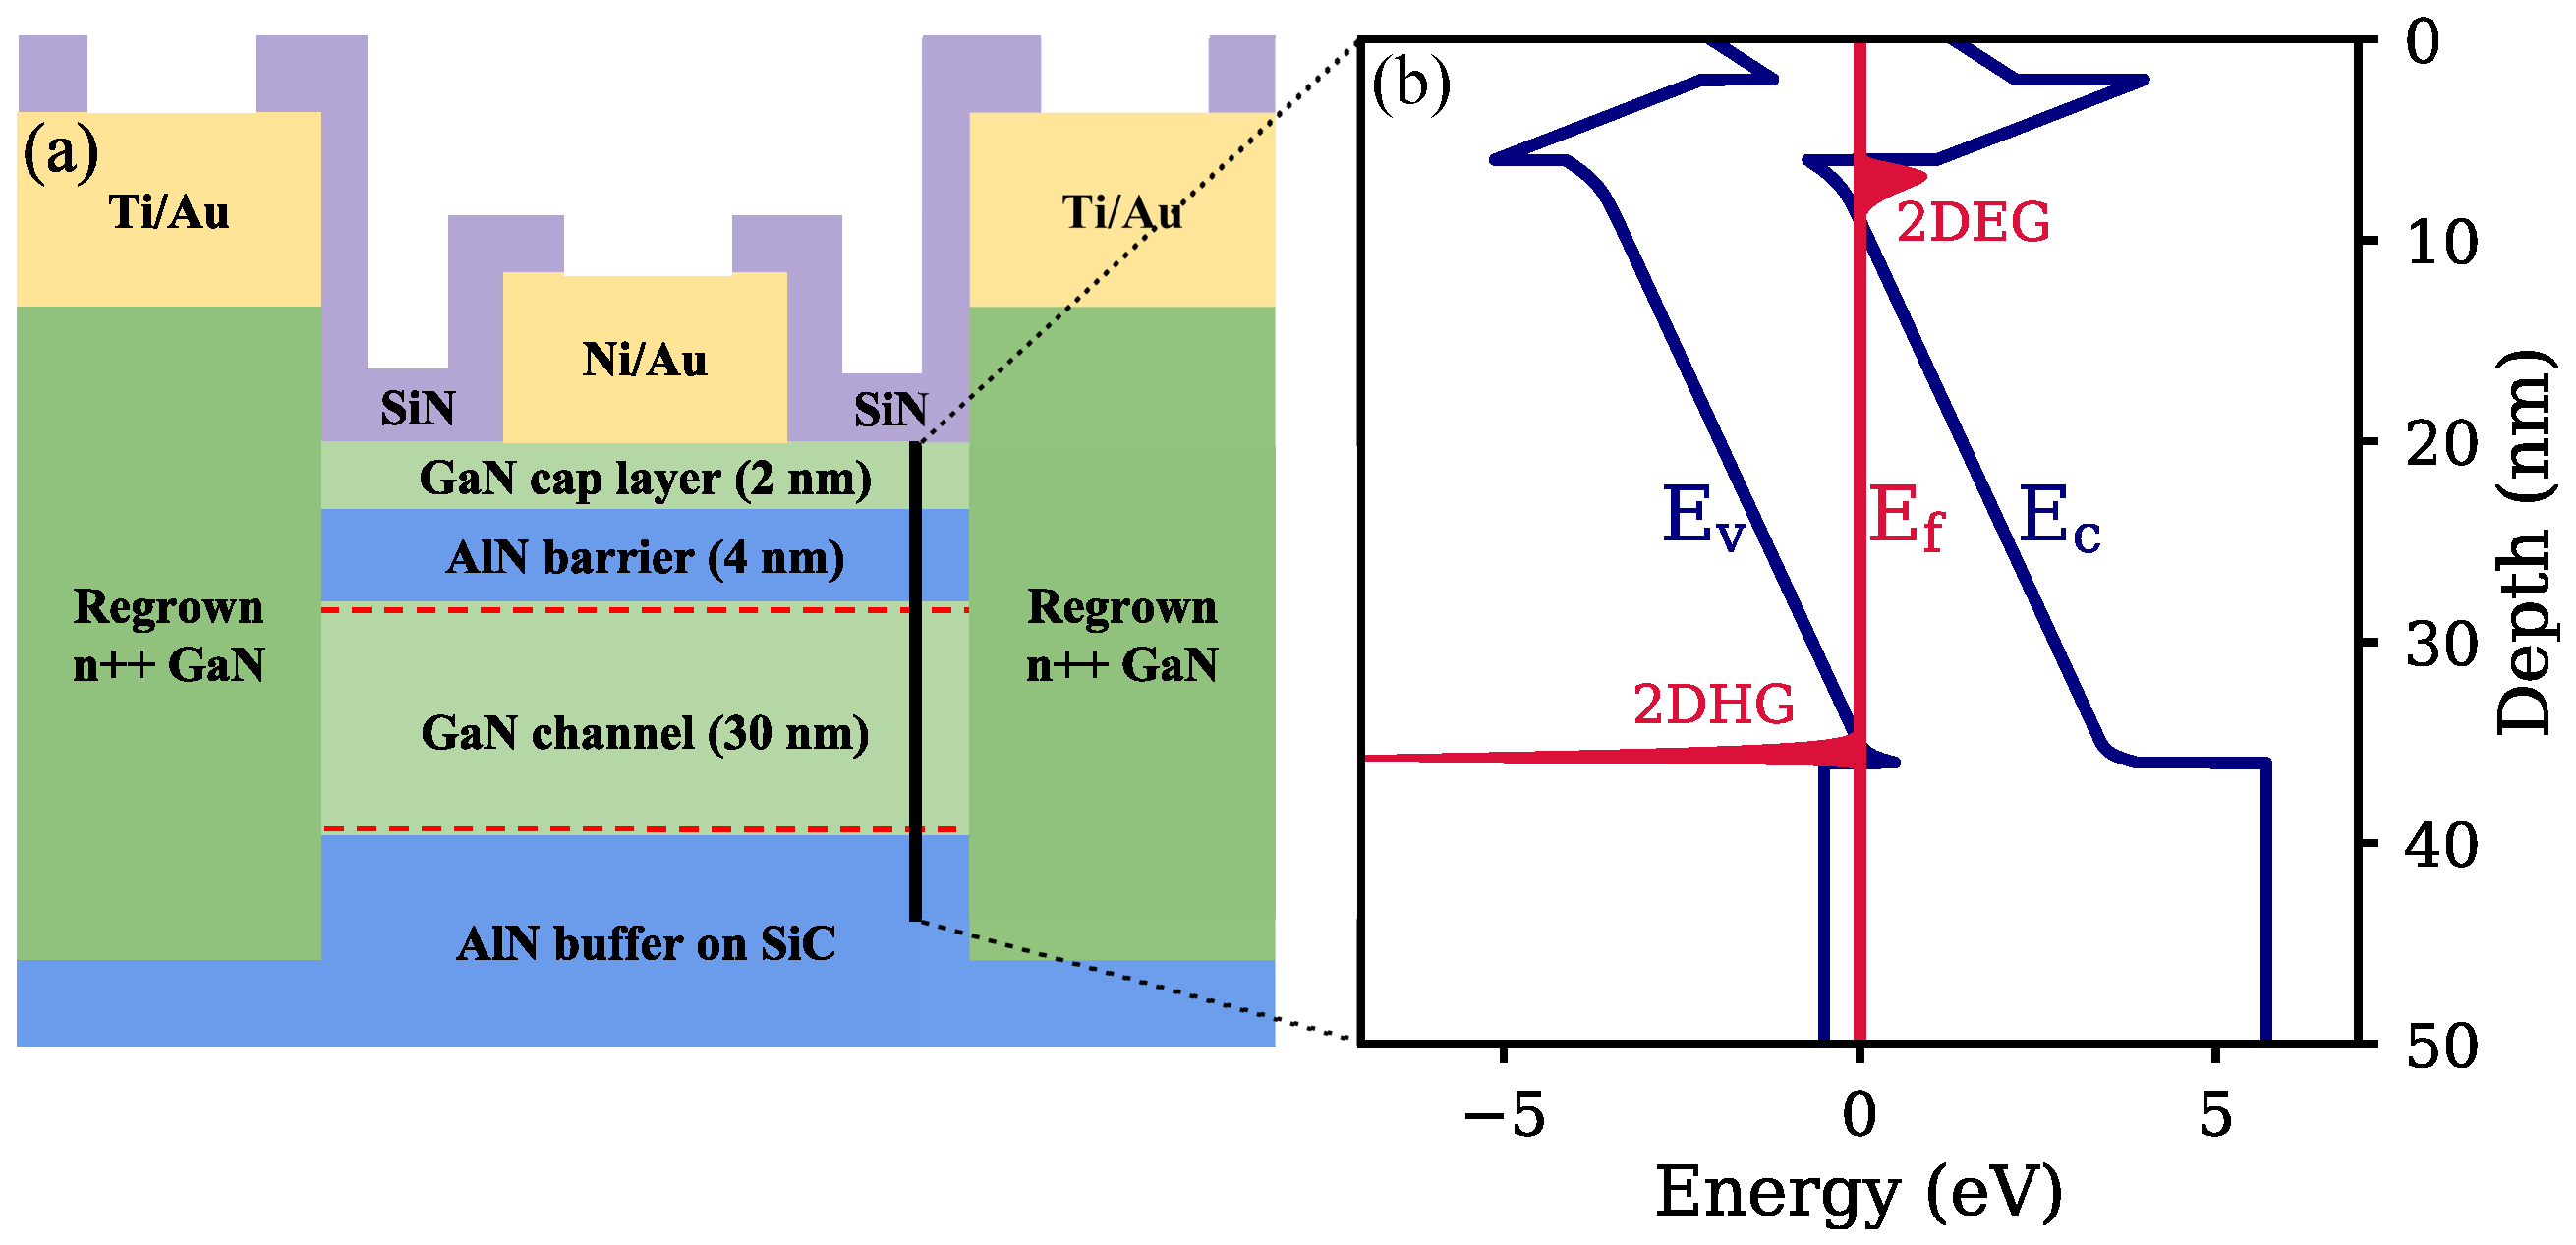
\includegraphics[width=\columnwidth]{Figure1.eps}
\caption{(a) Cross-sectional representation of a processed QW HEMT, and (b) corresponding energy band diagram simulated by 1D Poisson. }
\label{fig:epi}
\end{figure}

\begin{figure*}[!t]
\centering
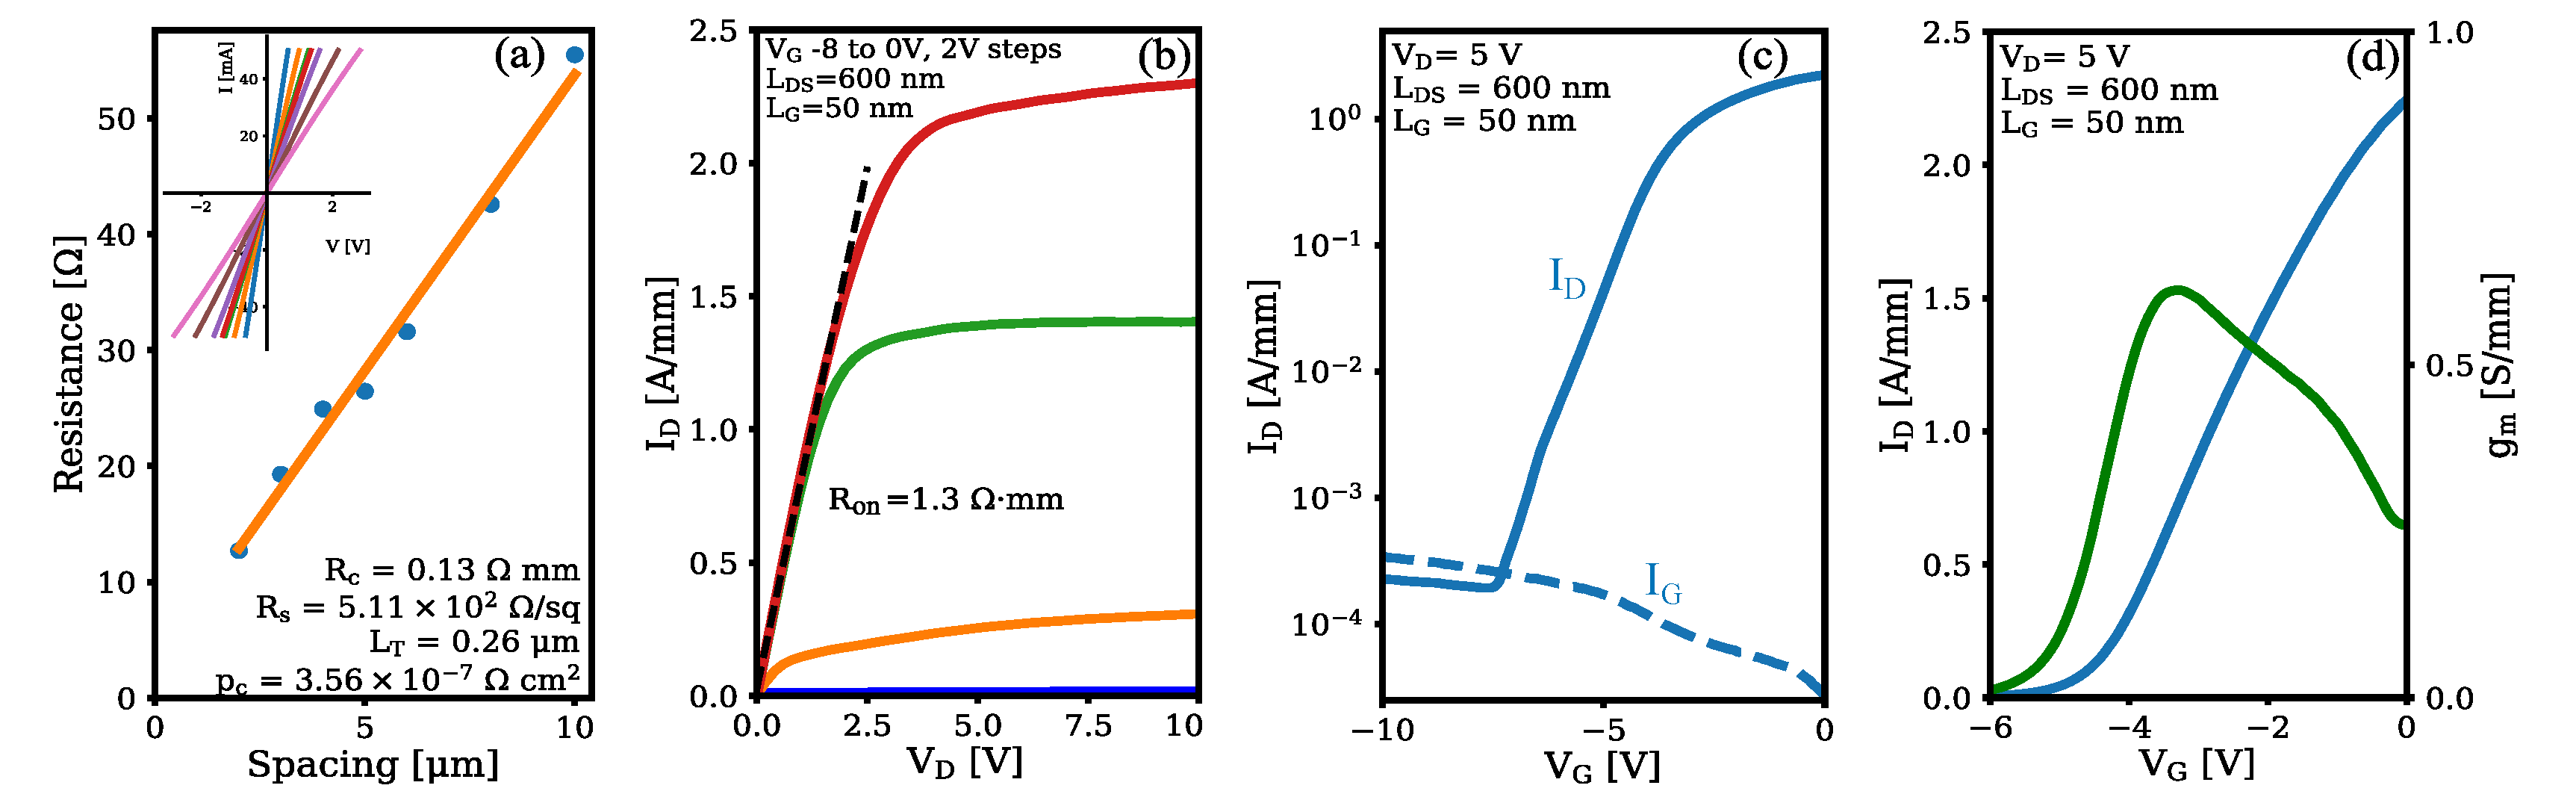
\includegraphics[width=\textwidth]{Figure2_shorter.eps}
\caption{(a) Linear TLM analysis of the non-annealed Ti/Au ohmic contacts to the regrown GaN. (b) $\mathrm{I_DV_D}$ curves demonstrating current saturation for $\mathrm{I_D}\sim$2.3 A/mm with low $\mathrm{R_{on}}$ = 1.3 $\Omega\cdot$mm. (c) Log-scale transfer curves showing on/off ratio of $\mathrm{10^4}$ limited by gate leakage current. (d) Linear transfer curves reveal peak $\mathrm{g_m}$ = 0.6 S/mm, the highest transconductance reported for QW HEMTs. }
\label{fig:IdVg}
\end{figure*}

\section{Device Fabrication}
The AlN/GaN/AlN epitaxial structures were grown by plasma-assisted molecular beam epitaxy (MBE) on semi-insulating 6H silicon carbide substrates. The heterostructure consists of a 350 nm AlN buffer layer, a 30 nm GaN channel, a 4 nm AlN barrier, and a 2 nm GaN passivation layer as shown in Fig. 1(a). Room temperature Hall-effect measurements prior to device fabrication showed a two-dimensional electron gas (2DEG) sheet concentration of 2.9 $\cdot$ $\mathrm{10^{13}}$ $\mathrm{cm^{-2}}$ and electron mobility of 630 $\mathrm{cm^2}$/V·s, corresponding to a sheet resistance of 340 $\Omega$/sq. An energy band diagram of the as-grown heterostructure simulated via self-consistent solution of the Poisson and Schrodinger equations [9] is shown in Fig. 1(b) shows the formation of a 2DEG at the top AlN/GaN heterojunction. The simulation also indicates the formation of a 2D hole gas (2DHG) at the bottom GaN/AlN heterojunction. The 2DHG has been experimentally detected earlier via terahertz spectroscopy [8]. The effects of the possible 2DHG on HEMT performance are under investigation and left as a topic of future work.

The device fabrication used a realigned gate-last process. The heterostructure was patterned with a $\mathrm{SiO_2}$/chromium hard mask and etched via $\mathrm{BCl_3}$ inductively coupled plasma (ICP) to expose the 2DEG sidewall. The sample was loaded back into the MBE, and regrown n++ GaN ($\mathrm{N_D}\sim10^{20} \mathrm{cm^{-3}}$) source/drain contacts were formed. The $\mathrm{SiO_2}$/Cr mask was removed via HF, and device isolation was achieved by another $\mathrm{BCl_3}$ ICP etch that extended 20 nm into the AlN buffer. Ti/Au (50/50 nm) non-alloyed ohmic contacts were deposited by e-beam evaporation on top of the regrown GaN source/drain regions. Long-channel gates were patterned by photolithography, and Ni/Au (50/50 nm) Schottky contacts were deposited by e-beam evaporation directly on the sample surface. Sub-micron channel devices were patterned for RF gates using electron beam lithography (EBL) with a PMMA bilayer. Ni/Au (20/50 nm) Schottky contacts were deposited via e-beam evaporation directly on the sample surface. Gate lengths as short as 40 nm were observed via SEM, shown in Fig. 4(a). No field plate was implemented. The HEMTs were then passivated with low-power, plasma-enhanced chemical vapor deposition (PECVD) silicon nitride with a thickness of 40 nm. Contact holes were formed in the silicon nitride by 6:1 BOE etching to allow probing of the ohmic and gate contact pads. The final HEMT cross-section is shown in Fig. 1(a).

\begin{figure}[!b]
\centering
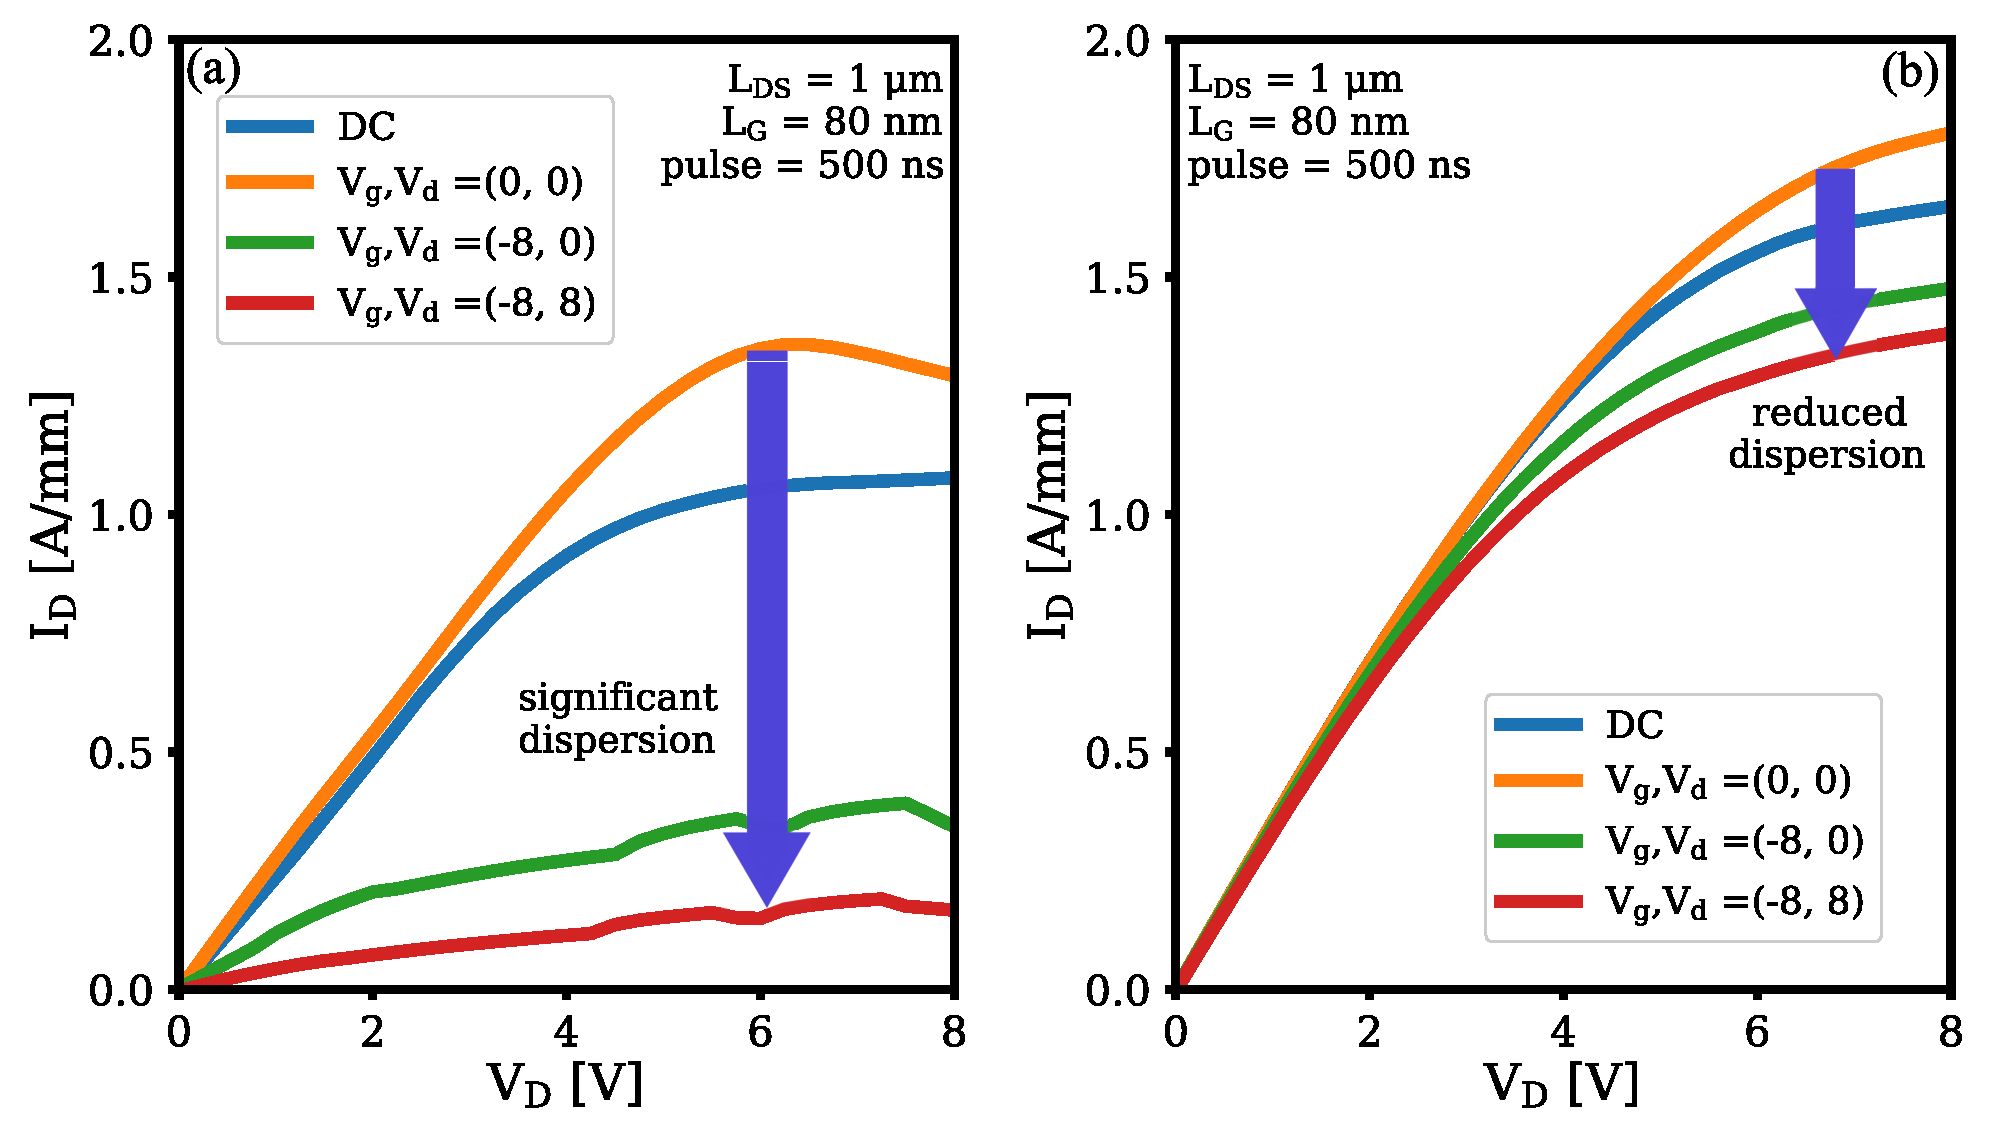
\includegraphics[width=\columnwidth]{Figure3.eps}
\caption{Pulsed $\mathrm{I_D-V_{DS}}$ measurements with a 500 ns pulse-width and 1 ms period. (a) Prior to silicon nitride passivation, pulsed $\mathrm{I_DV_D}$ revealed significant dispersion. (b) After SiN deposition, the dispersion has reduced to levels acceptable for breakdown measurements. }
\label{fig:pulsed}
\end{figure}

\section{Experimental Results and Discussion}
\label{sec:Experimental Results and Discussion}
After device fabrication, transfer-length method (TLM) patterns were measured in multiple locations across the sample, revealing excellent ohmic contact to the 2DEG with a contact resistance of $\mathrm{R_c}$ = 0.13 $\Omega\cdot$⋅mm, shown in Fig. 2(a). Hall-effect measurements at room temperature after fabrication revealed a 2DEG sheet concentration of 3 $\cdot$ $\mathrm{10^{13}}$ $\mathrm{cm^{-2}}$ and an electron mobility of 410 $\mathrm{cm^2}$/V·s, resulting in a sheet resistance of 510 $\Omega$/sq. The sheet resistance increased 50\% from its as-grown value, likely due to surface damage induced during the fabrication process and could be potentially avoided by changing the $\mathrm{SiO_2}$ deposition process. Transfer I-V characteristics reveal an $\mathrm{I_{on}}/\mathrm{I_{off}}$ = $\mathrm{10^4}$ (this value was $\mathrm{10^9}$ before passivation) with a peak transconductance of 0.6 S/mm, as shown in Fig. 2(c, d). This is the highest transconductance reported for devices on the AlN/GaN/AlN heterostructure platform and shows their high promise. The output characteristics, plotted in Fig. 2(b), show a drain current of $\sim$2.3 A/mm with excellent saturation and on-resistance of 1.3 $\Omega\cdot$mm.

\begin{figure*}[!t]
\centering
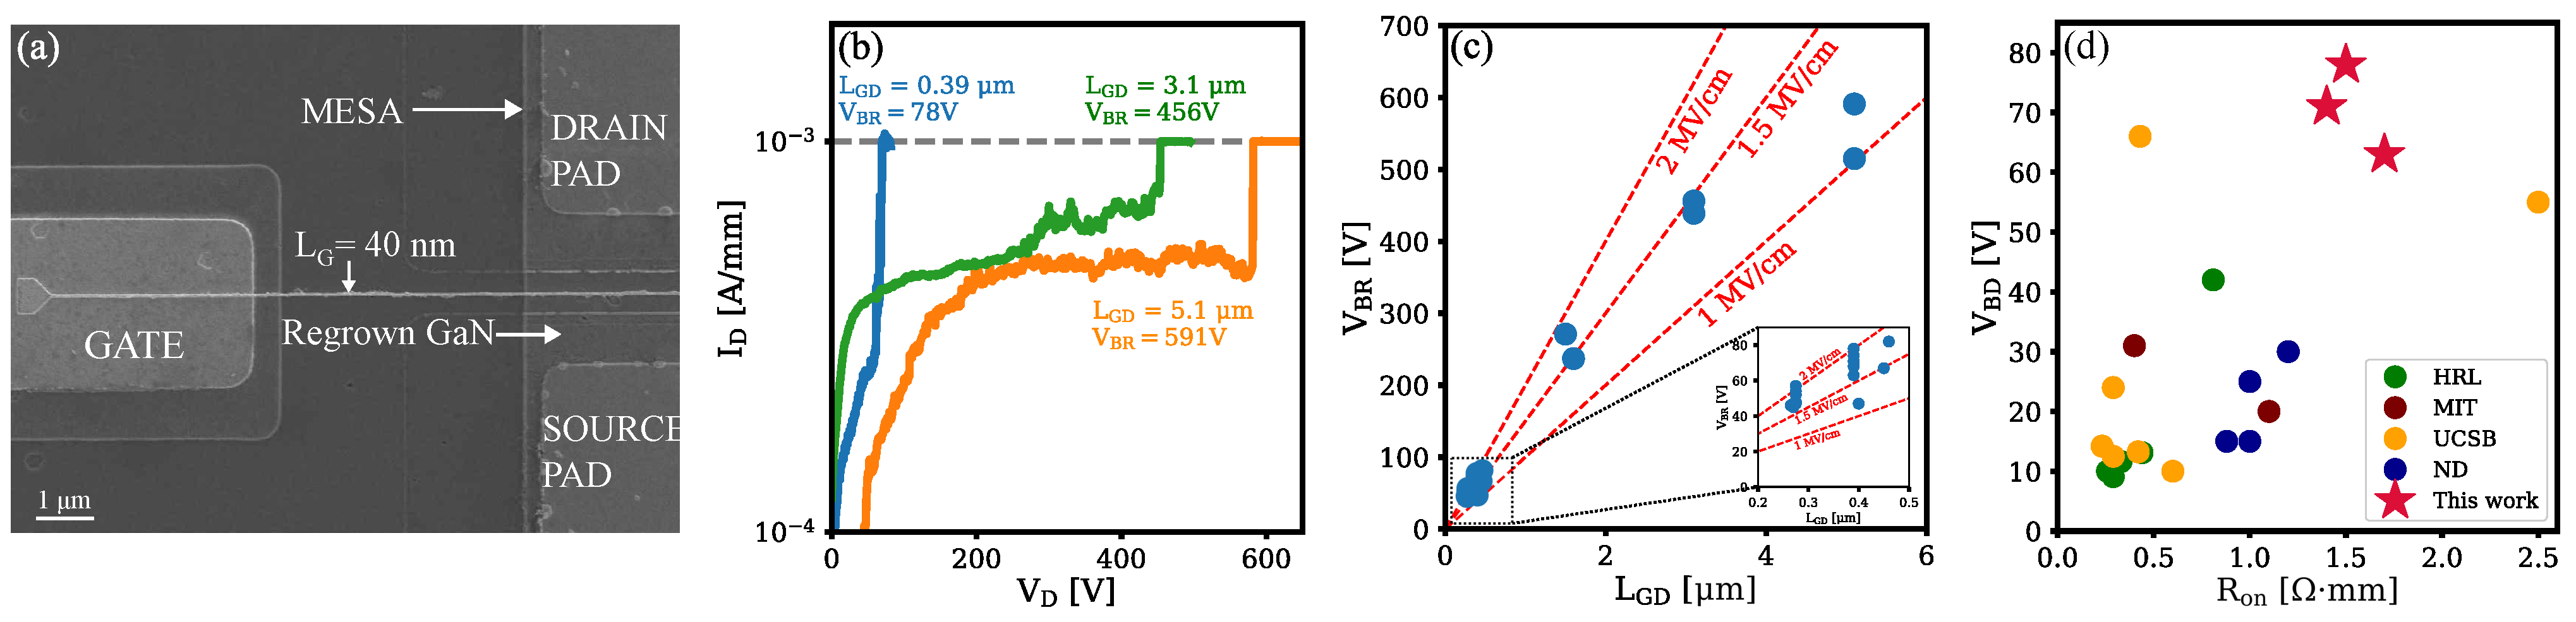
\includegraphics[width=\textwidth]{Figure4_withSEM.eps}
\caption{ (a) SEM image of a short-channel QW HEMT with $\mathrm{L_G}$ = 40 nm. (b) Hard breakdown for three HEMTs with varied gate-drain separations. (c) Breakdown voltage scaling as a function of gate-drain separation ranging from 0.27 to 5.1 $\mu$m. (d) $\mathrm{V_{BD}}$ and $\mathrm{R_{on}}$ benchmark plot comparing the QW HEMTs to state-of-the-art GaN HEMTs. }
\label{fig:benchmark}
\end{figure*}


Pulsed $\mathrm{I_D-V_{DS}}$ measurements were performed before and after SiN passivation to ensure the elimination of any virtual gate that may impact the effective gate-drain distance. Dispersion was found to be significantly reduced by SiN passivation, but not eliminated, as shown in Fig. 3(a) for before passivation and 3(b) after. Further optimization of the SiN deposition process should help improve the dispersion. To investigate breakdown characteristics, the gate voltage was set below the threshold voltage (typically $\mathrm{V_G}$ = -8 V), and $\mathrm{V_{DS}}$ was increased until HEMT breakdown occurred. The breakdown voltage metric is defined as $\mathrm{I_D}$ $\geq$ 1 mA/mm. QW HEMTs were tested for gate-drain lengths ($\mathrm{L_{GD}}$) ranging from 270 nm to 5.1 $\mu$m. The devices were covered in Fluorinert during the measurement process.

Fig. 4(b) shows the three terminal off-state breakdown of three QW HEMTs with varied gate-drain distances. Among all devices, the highest breakdown voltage observed is $\mathrm{V_{BD}}$ = 591 V ($\mathrm{L_{GD}}$ = 5.1 $\mu$m), corresponding to an average electric field ($\mathrm{E_{BD}}$) of 1.16 MV/cm. All measured devices had average electric fields above 1 MV/cm at breakdown. During the measurement process and prior to breakdown, the gate current is found to be roughly equal to the drain current. This indicates the off-state drain current and breakdown is dominated by gate-drain leakage and not avalanche or channel breakdown, and is far from the material limits. Post-breakdown, the device is visibly damaged on the drain side of the gate, representing catastrophic breakdown occurring within the barrier/channel region of the device.

To explore the potential for high-frequency applications, sub-micron channel lengths were examined for breakdown. A breakdown voltage of 78 V was measured for a HEMT with 390 nm gate-drain distance. This corresponds to an effective breakdown field of 2 MV/cm. This is among the largest breakdown voltages reported for a sub-micron channel nitride HEMT, demonstrating the potential of QW HEMTs for extremely high-power operation in RF applications. Fig. 4(c) shows the scaling of breakdown voltage as a function of $\mathrm{L_{GD}}$. The breakdown voltage does not quite scale linearly with $\mathrm{L_{GD}}$, which is expected due to the non-uniform distribution of the E-field within the channel.

\section{Conclusions and Benchmarking}
The breakdown voltages and on-resistances measured in this work are benchmarked against state-of-the-art GaN HEMTs [10]-[25] in Fig. 4(d). All devices shown have submicron $\mathrm{L_{GD}}$, and no field plate. The breakdown voltage for QW HEMTs is among the highest reported for sub-micron channel devices, while the on-resistance still lags behind its GaN counterparts. The moderate on-resistance is likely due to the high sheet resistance of the processed sample. This is currently being addressed by growth optimization to reduce the initial sheet resistance, and by process optimization to prevent any increase in the as-grown sheet resistance.

In this letter, the breakdown characteristics of strained AlN/GaN/AlN quantum well HEMTs were explored for the first time. The fabricated devices demonstrated excellent DC characteristics, with $\mathrm{R_c}$ = 0.13 $\Omega\cdot$mm, $\mathrm{I_{Dsat}}$ = 2.3 A/mm, and peak $\mathrm{g_m}$ = 0.6 S/mm. HEMTs with $\mathrm{L_{GD}}$ ranging from 270 nm to 5.1 $\mu$m were tested for breakdown characteristics, and a clear dependence of breakdown voltage on gate-drain distance is observed. Outstanding breakdown voltage is observed across all gate-drain lengths, most notably for sub-micron channel devices, in which a breakdown voltage of 78 V was measured for a device with $\mathrm{L_{GD}}$ = 390 nm, $\mathrm{L_{SD}}$ = 800 nm. The high breakdown voltage and decent on-resistance demonstrate QW HEMTs as a viable platform and potential successor to AlGaN/GaN HEMTs for future high-power RF electronics.

\vfill

% Just to move references to the fourth page so it's clear
% that my document ends at 2 2/3 pages
{\color{white}
\pagebreak
%Document less than 2 2/3 pages.\pagebreak
%Document less than 2 2/3 pages.\pagebreak
%Document less than 2 2/3 pages.\pagebreak
}
\IEEEtriggeratref{12}

\bibliographystyle{IEEEtran}
%\bibliography{link}

\begin{thebibliography}{00}

\bibitem{b1} M. Danilovic, Z. Chen, R. Wang, F. Luo, D. Boroyevich, P. Mattavelli, "Evaluation of the switching characteristics of a Gallium-Nitride transistor", in Proc. IEEE Energy Conversion Congress and Exposition 2011, pp. 2681-2688, 17-22 Sept. 2011.

\bibitem{b2} R. Rounds, B. Sarkar, A. Klump, C. Hartmann, T. Nagashima, R. Kirste, A. Franke, M. Bickermann, Y. Kumagai, Z. Sitar, R. Collazo, "Thermal conductivity of single-crystalline AlN", Appl. Phys. Express, vol. 11, no. 7, p. 071001, 2018.

\bibitem{b3} G. Li, R. Wang, J. Guo, J. Verma, Z. Hu, Y. Yue, F. Faria, Y. Cao, M. Kelly, T. Kosel, H. G. Xing, D. Jena, "Ultrathin Body GaN-On-Insulator Quantum Well FETs with Regrown Contacts",  IEEE Electron Device Lett., vol. 33, no. 5, p. 661, May 2012.

\bibitem{b4} S.M. Islam, M. Qi, B. Song, K. Nomoto, V. Protasenko, J. Wang, S. Rouvimov, P. Fay, H. G. Xing, D. Jena, "First Demonstration of Strained AlN/GaN/AlN Quantum Well FETs on SiC", DRC 2016.

\bibitem{b5} M. Qi, G. Li, S. Ganguly, P. Zhao, X. Yan, J. Verma, B. Song, M. Zhu, K. Nomoto, H. G. Xing, D. Jena, "Strained GaN quantum-well FETs on single crystal bulk AlN substrates", Appl. Phys. Lett. 110, 063501 (2017).

\bibitem{b6} G. Li, R. Wang, B. Song, J. Verma, Y. Cao, S. Ganguly, A. Verma, J. Guo, H. G. Xing, D. Jena, "Polarization-Induced GaN-on-Insulator E/D Mode p-Channel Heterostructure FETs", IEEE Electron Device Lett., vol. 34, no. 7, p. 852, July 2013.

\bibitem{b7} S. J. Bader, R. Chaudhuri, K. Nomoto, A. Hickman, Z. Chen, H. W. Then, D. A. Mueller, H. G. Xing, D. Jena, "Gate-Recessed E-mode p-Channel HFET With High On-Current Based on GaN/AlN 2D Hole Gas", IEEE Electron Device Lett., vol. 39, no. 12, p. 1848, December 2018.

\bibitem{b8} H. Condori Quispe, S. M. Islam, S. Bader, A. Chanana, K. Lee, R. Chaudhuri, A. Nahata, H. G. Xing, D. Jena, and B. Sensale-Rodriguez, "Terahertz spectroscopy of an electron-hole bilayer system in AlN/GaN/AlN quantum wells", Appl. Phys. Lett. 111, 073102 (2017)

\bibitem{b9} G. Snider, "1D Poisson".  Available: https://www3.nd.edu/~gsnider/.

\bibitem{b10} K. Shinohara, D. Regan, I. Milosavljevic, A. L. Corrion, D. F. Brown, P. J. Willadsen, C. Butler, A. Schmitz, S. Kim, V. Lee, A. Ohoka, P. M. Asbeck, M. Micovic., "Electron Velocity Enhancement in Laterally Scaled GaN DH-HEMTs with fT of 260 GHz", IEEE Electron Device Lett., vol. 32, no. 8, p. 1074, August 2011.

\bibitem{b11} K. Shinohara, A. Corrion, D. Regan, I. Milosavljevic, D. Brown, S. Burnham, P. J. Willadsen, C. Butler, A. Schmitz, D. Wheeler, A. Fung, and M. Micovic., "220GHz ft and 400GHz fmax in 40-nm GaN DH-HEMTs with Regrown Ohmic", IEDM Tech. Dig., p672, 2010.

\bibitem{b12} K. Shinohara, D. Regan, A. Corrion, D. Brown, S. Burnham, P.J. Willadsen, I. Alvarado- Rodriguez, M. Cunningham, C. Butler, A. Schmitz, S. Kim, B. Holden, D. Chang, V. Lee, A. Ohoka, P.M. Asbeck, and M. Micovic., "Deeply-Scaled Self-Aligned-Gate GaN DH-HEMTs with Ultrahigh Cutoff Frequency", IEDM Tech. Dig., p453, 2011.

\bibitem{b13} Y. Tang, K. Shinohara, D. Regan, A. Corrion, D. Brown, J. Wong, A. Schmitz, H. Fung, S. Kim, and M. Micovic., "Ultrahigh-Speed GaN High-Electron-Mobility Transistors With ft/fmax of 454/444 GHz",  IEEE Electron Device Lett., vol. 36, no. 6, p. 549, June 2015.

\bibitem{b14} J. W. Chung, W. E. Hoke, E. M. Chumbes T. Palacios, "AlGaN/GaN HEMT With 300-GHz fmax",  IEEE Electron Device Lett., vol. 31, no. 3, p. 195, March 2010

\bibitem{b15} T. Palacios, C.-S. Suh, A. Chakraborty, S. Keller, S. P. DenBaars, U. K. Mishra, "High-Performance E-Mode AlGaN/GaN HEMTs", IEEE Electron Device Lett., vol. 27, no. 6, p. 428, June 2006.

\bibitem{b16} D. S. Lee, O. Laboutin, Y. Cao, W. Johnson, E. Beam, A. Ketterson, M. Schuette, P. Saunier, D. Kopp, P. Fay, T. Palacios, "317 GHz InAlGaN/GaN HEMTs With Extremely Low On-Resistance", Phys. Status Solidi C 10, No. 5, 827– 830 (2013)

\bibitem{b17} Nidhi, S. Dasgupta, D. F. Brown, S. Keller, J. S. Speck, U. K. Mishra, "N-Polar GaN-Based Highly Scaled Self-Aligned MIS-HEMTs with State-of-the-art fT-Lg Product of 16.8GHz-um", IEDM Tech. Dig., p955, 2009.

\bibitem{b18} Nidhi, S. Dasgupta, J. Lu, J. S. Speck, U. K. Mishra, "Self-aligned N-polar GaN/InAlN HEMTs with Record Extrinsic Transconductance of 1105 mS/mm",  IEEE Electron Device Lett., vol. 33, no. 6, p. 794, June 2012.

\bibitem{b19} D. J. Denninghoff, S. Dasgupta, J. Lu, S. Keller, U. K. Mishra, "Design of High-Aspect-Ratio T-Gates on N-Polar GaN/AlGaN MIS-HEMTs for High fmax",  IEEE Electron Device Lett., vol. 33, no. 6, p. 785, June 2012.

\bibitem{b20} D. Denninghoff, J. Lu, E. Ahmadi, S. Keller, U. K. Mishra, "N-polar GaN/InAlN MIS-HEMT with 400-GHz fmax", DRC Tech. Dig., p. 151, 2012.

\bibitem{b21} D. Denninghoff, J. Lu, M. Laurent, E. Ahmadi, S. Keller and U. K. Mishra, "N-polar GaN/InAlN/AlGaN MIS-HEMTs with 1.89 S/mm extrinsic transconductance, 4 A/mm drain current, 204 GHz fTand 405 GHz fmax", DRC Tech. Dig., p. 197, 2013.

\bibitem{b22} B. Romanczyk , S. Wienecke , M. Guidry, H. Li, E. Ahmadi, X. Zheng , S. Keller, and U. K. Mishra, "Demonstration of Constant 8 W/mm Power Density at 10, 30, and 94 GHz in State-of-the-Art Millimeter-Wave N-Polar GaN MISHEMTs", IEEE Transactions on Electron Devices, vol. 65, no. 1, p. 45,  January 2018

\bibitem{b23} Y. Yue, Z. Hu, J. Guo, B. Sensale-Rodriguez, G. Li, R. Wang, F. Faria, T. Fang, B. Song, S. Guo, T. Kosel, G. Snider, P. Fay, D. Jena, and H. Xing, "InAlN/AlN/GaN HEMTs With Regrown Ohmic Contacts and fT of 370 GHz", IEEE Electron Device Lett., vol. 33, no. 7, p. 988, July 2012.

\bibitem{b24} B. Sensale-Rodriguez, J. Guo, R. Wang, J. Verma, G. Li, T. Fang, E. Beam, A. Ketterson, M. Schuette, P. Saunier, X. Gao, S. Guo, G. Snider, P. Fay, D. Jena, H. G. Xing, "Time delay analysis in high speed gate-recessed E-mode InAlN HEMTs", Solid-State Electronics, 80, p. 67, 2013.

\bibitem{b25} R. Wang, G. Li, G. Karbasian, J. Guo, F. Faria, Z. Hu, Y. Yue, J. Verma, O. Laboutin, Y. Cao, W. Johnson, G. Snider, P. Fay, D. Jena, H. G. Xing, "InGaN Channel High-Electron-Mobility Transistors with InAlGaN Barrier and ft/fmax of 260/220 GHz", Applied Physics Express, 6, p. 16503, 2013.

\end{thebibliography}



\end{document}


